\documentclass[12pt,a4paper]{article}
\usepackage[T2A]{fontenc}
\usepackage[utf8]{inputenc}
\usepackage[russian]{babel}
\usepackage{amsmath}
\usepackage{amssymb}
\usepackage{graphicx}
\usepackage{floatrow}
\usepackage{booktabs}
\usepackage{wrapfig}
\usepackage{lipsum}
\usepackage{subcaption}


\newcommand{\figref}[1]{(См. рис. \ref{#1})}
\newcommand{\secref}[1]{(См. раздел. \ref{#1})}

\newcommand{\e}[1]{\text{$\cdot10^{#1}$}}



\author{\normalsize Выполнил: Голубович Тимур, группа Б01-108 \\
	\normalsize 16.03.2022}
\date{}



\usepackage{float}
\restylefloat{table}
\title
{
	\large Отчет о выполнении лабораторной работы 1.3.3 \\
	\Large Определение вязкости воздуха по скорости течения через тонкие трубки \\ 
}


\begin{document}
	\maketitle
	
\subsection*{Цель работы} Экспериментально выявить участок сформированного течения, определить режимы ламинарного и турбулентного течения; определить число Рейнольдса.

\subsection*{Теоретическое введение}
Рассмотрим движение вязкой жидкости или газа по трубке круглого сечения. При малых скоростях потока движение оказывается ламинарным (слоистым), скорости частиц меняются по радиусу и направлены вдоль оси трубки. С увеличением скорости потока движение становится турбулентным, и слои перемешиваются. При турбулентном движении скорость в каждой точке быстро меняет величину и направление, сохраняется только средняя величина скорости.
Характер движения газа (или жидкости) в трубке определяется безразмерным числом Рейнольдса:

\[Re = \dfrac{\upsilon r \rho}{\eta} \text{  } \text{  } \text{  }(1)\]

где $\upsilon$ - скорость потока, $r$ - радиус трубки, $\rho$ - плотность движущейся среды, $\eta$ - вязкость. В гладких трубах круглого сечения переход от ламинарного движения к турбулентному происходит при $Re \approx 1000$

При ламинарном течении объем газа $V$, протекающий за время $t$ по трубе длиной $l$, определяется формулой Пуазейля:
\[Q_V = \dfrac{\pi r^4}{8 l \eta}(P_1 - P_2) \text{  } \text{  } \text{  }(2)\]
В этой формуле $P_1 - P_2$ - разность давлений в двух выбранных сечениях 1 и 2, расстояние между которыми равно $l$. Велечину $Q$ обычно называют расходом. Формула (2) позволяет определять вязкость газа по его расходу.

Отметим условия, при которых справедлива формула (2). Прежде всего необходимо, чтобы с достаточным запасом выполнялось неравенство $Re < 1000$. Необходимо также, чтобы при течении не происходило существенного изменения удельного объема газа (при выводе формулы удельный объем считался постоянным). Для жидкости это предположение выполняется практически всегда, а для газа - лишь в тех случаях, когда перепад давлений вдоль трубки мал по сравнению с самим давлением. В нашем случае давление газа равно атмосферному ($10^3$ см вод. ст.), а перепад давлений составляет не более 10 см вод. ст., то есть менее $1\%$ от атмосферного. Формула (2) выводится для участков трубки, на которых закон распределения скоростей газа по сечению не меняется при движении вдоль потока.

\begin{figure}[H]
	\begin{center}
		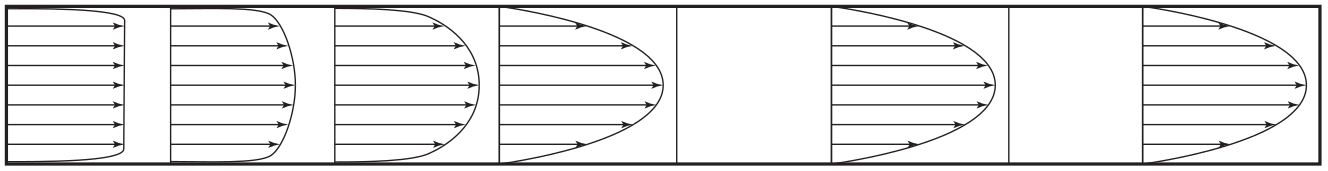
\includegraphics[width=12cm]{src/potok.png}
	\end{center}
	\caption{Формирование потока газа в трубе круглого сечения}
	\label{img1}
\end{figure}	
	

При втекании газа в трубку из большого резервуара скорости слоев вначале постоянны по всему сечению (рис. 1). По мере продвижения газа по трубке картина распределения скоростей меняется, так как сила трения о стенку тормозит прилежащие к ней слои. Характерное для ламинарного течения параболическое распределение скоростей устанавливается на некотором расстоянии $a$ от входа в трубку, которое зависит от радиуса трубки $r$ и числа Рейнольдса по формуле
\[a \approx  0,2 r \cdot Re \text{ } \text{ } \text{ } (3)\]
Градиент давления на участке формирования потока оказывается большим, чем на участке с установившимся ламинарным течением, что позволяет разделить эти участки экспериментально. Формула (3) дает возможность оценить длину участка формирования.
\subsection*{Экспериментальная установка}

\begin{figure}[H]
	\begin{center}
		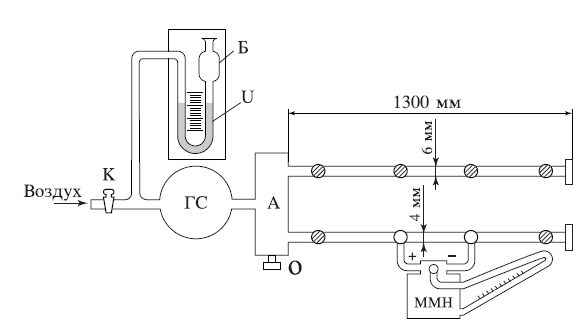
\includegraphics[width=12cm]{src/scheme.png}
	\end{center}
	\caption{Схема установки для определения вязкости воздуха}
	\label{img2}
\end{figure}	

  Измерения производятся на экспериментальной установке, схема которой изображена на рис. 2. Поток воздуха под давлением, несколько превышающим атмосферное (на 5-7 см вод. ст.), через газовый счетчик ГС поступает в резервуар А, к которому припаяны тонкие металлические трубки. Примерные размеры трубок указаны на рисунке (точные размеры обозначены на установке). Обе трубки на концах снабжены заглушками, не пропускающими воздух. Во время измерений заглушка открывается только на рабочей трубке; конец другой трубки должен быть плотно закрыт. Перед входом в газосчётчик поставлена U-образная трубка, наполовину заполненная водой. Она выполняет две задачи. Первая - измерение давления газа на входе в газосчётчик. Вторая - предохранение газосчётчика от выхода из строя. Дело в том, что газосчётчик устойчиво работает, если давление газа на его входе не превышает 600 мм водяного столба. Высота U-образной трубки примерно 600 мм, поэтому, когда давление на входе в счётчик превышает 600 мм водяного столба,вода из U-образной трубки выплёскивается в защитный баллон Б и, создавая шум, привлекает к себе внимание экспериментатора. 
  
\subsection*{Ход работы}


Проведя измерения, занесем точки в таблицу \ref{tab:data}. Построим графики полученных зависимостей (см. рис. \ref{fig:pot}). 


\begin{table}
\begin{floatrow}
\input{Линеаризация}
\input{Линеаризация2}
\end{floatrow}
\end{table}



\begin{figure}
	\centering
	\includegraphics[width=1\linewidth]{"P(T)"}
	\caption{Температура от давления}
	\label{fig:pot}
\end{figure}

\begin{figure}
	\centering
	\includegraphics[width=1\linewidth]{"lnP(T)"}
	\caption{Линеаризация $\ln{P}(\frac{1}{T})$}
	\label{fig:lnpot}
\end{figure}

\begin{figure}
	\centering
	\includegraphics[width=1\linewidth]{"dpdt"}
	\caption{Линеаризация $\frac{dP}{dT}(\frac{P}{T^2})$}
	\label{fig:dpdt}
\end{figure}



\begin{table}
	\caption{Обработка $\ln{p}(\frac{1}{T})$}
	\label{tab:stat}
	\centering
	\footnotesize
	\begin{tabular}{l|ccccccccc}
		\toprule
		$ $ & $\overline{x}$ & $\sigma_x^2$ & $\overline{y}$ & $\sigma_y^2$ & $r_{xy}$ & $A$ & $\Delta A$ & $B$ & $\Delta B$ \\ \midrule
		Нагрев & 3.29e-03 & 3.51e-09 & 3.40 & 1.06e-01 & -1.93e-05 & -5488.87 & 115.05 & 21.46 & 0.38 \\ 
		Охлаждение & 3.29e-03 & 3.51e-09 & 3.46 & 1.01e-01 & -1.88e-05 & -5365.12 & 101.15 & 21.10 & 0.33 \\ \bottomrule
	\end{tabular}
\end{table}


\begin{table}
	\caption{Обработка $\frac{dP}{dT}(\frac{P}{T^2})$}
	\label{tab:dpstat}
	\centering
	\footnotesize
	\begin{tabular}{l|ccccccccc}
		\toprule
		$ $ & $\overline{x}$ & $\sigma_x^2$ & $\overline{y}$ & $\sigma_y^2$ & $r_{xy}$ & $A$ & $\Delta A$ & $B$ & $\Delta B$ \\ \midrule
		Нагрев & 3.39e-04 & 9.10e-09 & 1.92 & 3.66e-01 & 5.76e-05 & 6326.01 & 236.72 & -0.22 & 0.08 \\ 
		Охлаждение & 3.56e-04 & 9.62e-09 & 1.85 & 3.55e-01 & 5.82e-05 & 6053.28 & 257.56 & -0.30 & 0.10 \\ \bottomrule
	\end{tabular}
\end{table}


Перейдем к расчету зависимостей. Обработку проведем методом наименьших квадратов:

$$y = Ax + B,$$

где $$A = \frac{r_{xy}}{ \sigma_x^2},$$
$$B = \overline{y} - A\overline{x}.$$

Для оценки погрешностей используем следующие формулы:
$$\Delta A =  t_{n-1, p} \sqrt{\frac{1}{n-2} \left( \frac{\sigma_y^2}{\sigma_x^2} - A^2 \right)},$$
$$\Delta B = \Delta A \sqrt{\sigma_x^2 + \overline{x}^2},$$

где 
$n$ - количество измерений, $ t_{n-1, p}$ - коэффициент Стьюдента

Таким образом проведем две линеаризации (см. таблицы \ref{tab:linear} и \ref{tab:linear2}) используя зависимости:

$$\frac{dP}{dT} = \frac{L}{R} \cdot \frac{P}{T^2}$$
$$\ln{P} = -\frac{L}{R} \cdot \frac{1}{T} + C$$

Всю статистическую обработку занесем в таблицы \ref{tab:stat} и \ref{tab:dpstat}. Также построим графики зависимостей, для качественного анализа поведения (см. рис. \ref{fig:lnpot} и \ref{fig:dpdt})

Так как удельная теплота отличается от коэффициента наклона множителем, то относительная погрешность будет такой же. Откуда для молярных, а затем и удельных теплот парообразования получаем значения, которые занесем в таблицу \ref{tab:itog}. Молярная масса воды $\mu = 18.02 \frac{\text{г}}{\text{моль}}$



\subsection*{Вывод}


Из отчета видно, что на точность полученных результатов (см. таблицу \ref{tab:itog}) влияет не только ошибки проведения эксперимента, но последующая обработка: выбор зависимости для линеаризации, методы определения параметров. Во втором способе погрешность получается на порядок больше, чем в первом.


\begin{table}[H]
	\caption{Вывод}
	\label{tab:itog}
	\centering
	\footnotesize
	\begin{tabular}{l|r|r}
		\toprule
		$ $ & Нагрев, $\frac{\text{Дж}}{\text{кг}}$& Охлаждение, $\frac{\text{Дж}}{\text{кг}}$ \\ \midrule
		Линеаризация $\ln{p}(\frac{1}{T})$          & $(2.53 \pm 0.053)\e{6}$ & $(2.48 \pm 0.047)\e{6}$  \\ \midrule 
		Линеаризация $\frac{dP}{dT}(\frac{P}{T^2})$ & $(2.92 \pm 0.11)\e{6}$ & $(2.79 \pm 0.12)\e{6} $  \\ \midrule
		Табличная величина 							& $2.30\e{6} $ & $2.30\e{6} $  \\ 
		\bottomrule
	\end{tabular}
\end{table}

Учесть погрешность определения теплоемкостей в данном случае проблематично, т.к. метод наименьших квадратов дает значение ошибки именно случайную. А в случае с первой линеаризацией видно, что решающую роль должна иметь систематическая погрешность измерений.


Тем не менее полученные результаты более чем подтверждают теоретическую модель. Графики получаются линейными, а значения теплоты не сильно отличаются от табличных.
 



\end{document}